\documentclass{article}
\usepackage{civ}

\title{CIV102: Finals Review}
\author{QiLin Xue}
\date{Fall 2020}
\usepackage{physics}
\usepackage{siunitx}
\usepackage{mathrsfs}
\usepackage{ wasysym }

\usetikzlibrary{arrows}
\begin{document}

\maketitle
\section{Trust}
\begin{itemize}
    \item To be a safe bridge, we want to prevent tension/compression failure by demanding the cross sectional area be:
    \begin{equation}
        A \ge \frac{2F}{\sigma_y}
        \label{eq:}
    \end{equation}
    where $\sigma_y$ is the yield strength and for steel, it is the same for both compression and tension.
    \item To prevent compression members from buckling, the moment of inertia needs to be:
    \begin{equation}
        I \ge \frac{3FL^2}{\pi^2 E}
        \label{eq:}
    \end{equation}
    \item And we also demand the radius of gyration $r$ to be:
    \begin{equation}
        r \ge \frac{L}{200}
        \label{eq:}
    \end{equation}
    \item To use the method of virtual work, replace all applied forces with a single force $F^*$ at the location of interest and solve for the forces in all the members $P^*$. Then the displacement is:
    \begin{equation}
        \Delta = \frac{1}{F^*}\sum \frac{PP^* L}{AE}
        \label{eq:}
    \end{equation}
    \item For a point load at midspan, the frequency of oscillations is:
    \begin{equation}
        f_n = \frac{15.76}{\sqrt{\Delta}}
        \label{eq:}
    \end{equation}
    For a uniformly distributed load, we have:
    \begin{equation}
        f_n = \frac{17.76}{\sqrt{\Delta}}
        \label{eq:}
    \end{equation}
\end{itemize}
\section{Beem}
\begin{itemize}
    \item Navier's equation is:
    \begin{equation}
        \sigma = \frac{My}{I}
        \label{eq:}
    \end{equation}
    \item The curvature is:
    \begin{equation}
        \phi = \frac{M}{EI}
        \label{eq:}
    \end{equation}
    \item The change in slope between two points is given by the \textbf{first moment area theorem}:
    \begin{equation}
        \Delta_{AB} = \theta_B - \theta_A = \int_A^B \phi(x) \dd{x}
        \label{eq:}
    \end{equation}
    \item The \textbf{second moment area theorem} gives the deviation of point $D$ from the tangent drawn at point $T$ as:
    \begin{equation}
        \delta_{DT} = \int_D^T x\phi(x) \dd{x} = \bar{x}_{DT}\int_D^T\phi(x) \dd{x} = \sum \bar{x}\int \phi(x) \dd{x}
        \label{eq:}
    \end{equation}
    \item There are three scenarios when finding the deflection:
    \begin{itemize}
        \item Known horizontal tangent due to support: Find the deflection of the point of interest from the support condition.
        \item Known horizontal tangent due to symmetry: Find the deflection of the support from the point of interest.
        \item No known horizontal tangents: Find the deflection of support $C$ from the tangent drawn from the other support $A$. Find the deflection of the point of interest from support $A$. Use similar triangles to relate them together. To calculate the deflection of the support from $A$, we have:
        \begin{equation}
            \theta_A = \frac{\delta_{CA}}{L}
            \label{eq:}
        \end{equation}
        
    \end{itemize}
    \item Shear stresses are given by \textbf{Jourawski's equation}:
    \begin{equation}
        \tau = \frac{VQ}{Ib}
        \label{eq:}
    \end{equation}
    where:
    \begin{equation}
        Q = \int_{y_\text{bot}}^{y} y \dd{A} = \int_y^{y_\text{top}} y \dd{A} = \sum Ad
        \label{eq:}
    \end{equation}
    \item Plate buckling equations are given below:
    \begin{center}
        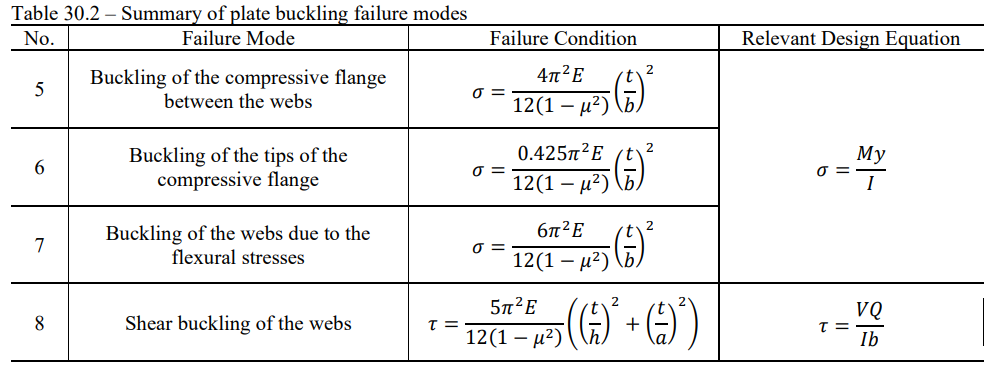
\includegraphics[width=0.8\linewidth]{plate_buckling.PNG}
    \end{center}
\end{itemize}
\section{Kuancrete}
\subsection{Properties}
\begin{itemize}
    \item The \textbf{concrete compressive strength} $f_c'$ and the \textbf{concrete tensile strength} $f_t'$ is related by the relationship:
    \begin{equation}
        f_t' = 0.33\sqrt{f_c'}
        \label{eq:}
    \end{equation}
    \item The Young's modulus of the concrete $E_c$ can be correlated to the compressive strength of concrete via:
    \begin{equation}
        E_c = 4730\sqrt{f_c'}
        \label{eq:}
    \end{equation}
    \item For \textit{reinforcing steel}, the Young's modulus is $E_s = 200,000\si{\mega\pascal}$ and the yield strength is $f_y = 400\si{\mega\pascal}$. 
    \item The \textbf{modular ratio} $n$ is given as:
    \begin{equation}
        n = \frac{E_s}{E_c}
        \label{eq:}
    \end{equation}
    \item The \textbf{quantity of longitudinal reinforcement} $\rho$ is given as:
    \begin{equation}
        \rho = \frac{A_s}{bd}
        \label{eq:}
    \end{equation}
    where $A_s$ is the area of the steel reinforcements, $b$ is the width of the cross sectional region of interest and $d$ is the distance from the top/bottom edge of the region of interest to the opposing reinforcements. Refer to the below diagram:
    \begin{center}
        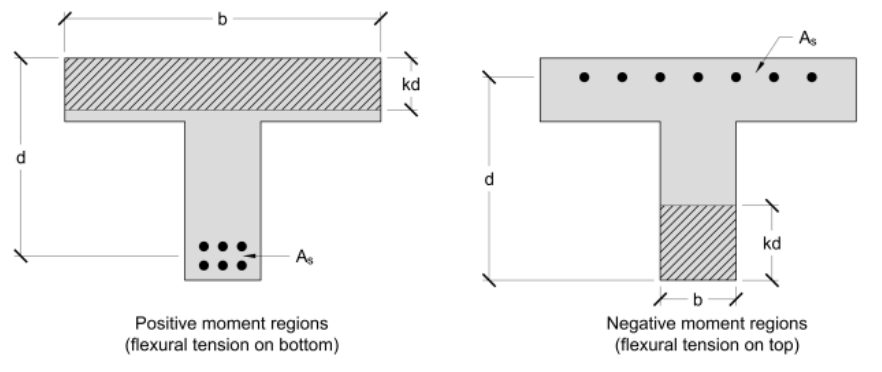
\includegraphics[width=0.7\linewidth]{concrete_cross_section.png}
    \end{center}
    \item The value of $k$ (scaling factor such that $kd$ is the distance from the extreme compression fibre to the neutral axis) is given as:
    \begin{equation}
        k = \sqrt{(n\rho)^2+2n\rho}-n\rho
        \label{eq:}
    \end{equation}
    \item The value of $j$ (scaling factor such that the \textbf{flexural lever} $jd$ is the vertical distance between the compressive and tensile forces) is given as:
    \begin{equation}
        j = 1 - \frac{1}{3}k
        \label{eq:}
    \end{equation}
    \item If the values of $k$ and $j$ are unknown, let $k=\frac{3}{8}$ and $j=\frac{7}{8}$.
\end{itemize}
\subsection{Flexural Stress Analysis}
\begin{itemize}
    \item The stress in the reinforcement $f_s$ is given by:
    \begin{equation}
        f_s = \frac{M}{A_sjd}
        \label{eq:}
    \end{equation}
    where $M$ is the bending moment carried by the member.
    \item The stress in the concrete $f_c$ is given by:
    \begin{equation}
        f_c = \frac{k}{1-k}\frac{M}{nA_sjd}
        \label{eq:}
    \end{equation}
    \item The maximum moment which can be carried by the member if it fails by yielding, $M_\text{yield}$ is given by:
    \begin{equation}
        M_\text{yield} = A_sf_yjd
        \label{eq:}
    \end{equation}
    \item Perform the following tests to see if the concrete is safe:
    \begin{itemize}
        \item $A_s \ge \frac{M}{0.6f_yjd}$
        \item $f_s \le 0.6f_y$
        \item $f_c \le 0.5f_c'$
    \end{itemize}
\end{itemize}
\subsection{Shear Stress Analysis}
\begin{itemize}
    \item The maximum shear stress $v$ we need to design for in a cracked concrete member occurs in its web, and is given by:
    \begin{equation}
        v = \frac{V}{b_wjd}
        \label{eq:}
    \end{equation}
    where $b_w$ is the effective web width.
    \item The shear stress $v_\text{max}$ that causes buckling to take place from the diagonal compression is given by:
    \begin{equation}
        v_\text{max} = 0.25f_c'
        \label{eq:}
    \end{equation}
    \item \textbf{With no shear reinforcement:} The shear strength of the concrete without shear reinforcement is given by:
    \begin{equation}
        V_c = \frac{230\sqrt{f_c'}}{1000+0.9d}b_wjd
        \label{eq:}
    \end{equation}
    \item \textbf{With shear reinforcement:} These are created with stirrups, and the shear strength in the concrete is given by:
    \begin{equation}
        V_c = 0.18\sqrt{f_c'}b_wjd
        \label{eq:}
    \end{equation}
    This equation is valid if:
    \begin{equation}
        \frac{A_vf_y}{b_ws} \ge 0.06\sqrt{f_c'}
        \label{eq:}
    \end{equation}
    where $A_v$ is the effective area of the stirrups. See the below diagram for different configurations:
    \begin{center}
        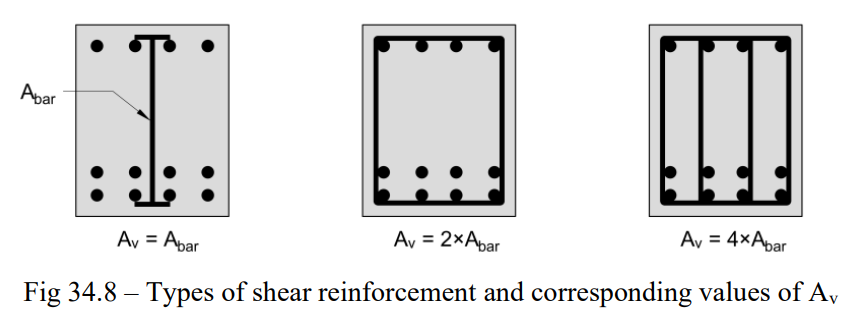
\includegraphics[width=0.8\linewidth]{stirrup_types.PNG}
    \end{center}
    If this is not satisfied, we can calculate $V_c$ using the equation with no shear reinforcements.
    \item If shear reinforcement is present, the maximum shear force carried in the truss is:
    \begin{equation}
        V_s = \frac{A_vf_yjd}{s}\cot(35^\circ)
        \label{eq:}
    \end{equation}
    where $s$ is the spacing of the shear reinforcement.
    \begin{center}
        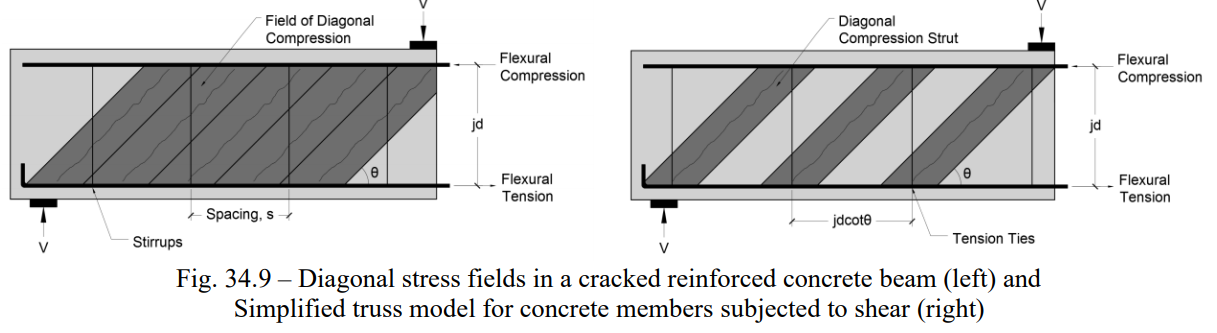
\includegraphics[width=\linewidth]{shear_truss.PNG}
    \end{center}
    \item The \textbf{shear strength} $V_r$ of the member is given by:
    \begin{equation}
        V_r = V_c + V_s
        \label{eq:}
    \end{equation}
    \item The limit at which concrete crushes is:
    \begin{equation}
        V_\text{max} = 0.25f_c'b_wjd
        \label{eq:}
    \end{equation}
    \item The concrete will fail when:
    \begin{equation}
        V \ge \min\{V_r, V_\text{max}\}
    \end{equation}
    \item For design, we want to pick $V_r$ to satisfy:
    \begin{equation}
        V_r = 0.5V_c + 0.6V_s \le 0.5 V_\text{max}
        \label{eq:}
    \end{equation}
    where the constants represent the factors of safety. If a given design is not safe, here are the things that can be tried:
    \begin{itemize}
        \item If $V \ge 0.5V_\text{max}$, the cross section needs to be resized.
        \item If $V \ge 0.5V_c$, then reinforcements need to be made.
        \item If $V \ge 0.5V_c + 0.6V_s$, then the spacing needs to be changed to:
        \begin{equation}
            s = \frac{0.6A_vf_yjd\cot(\theta)}{V-0.5\times 0.18\sqrt{f_c'}b_wjd}
            \label{eq:}
        \end{equation}
        
    \end{itemize}
    \begin{idea}
        In real life, cracks happen not at the highest shear, but instead a distance $d$ away from it. Therefore, the maximum shear force we are designing for is given by:
        \begin{equation}
            V_\text{design} = V_\text{support} - wd
            \label{eq:}
        \end{equation}
        where $w$ is the weight distribution. If $V_\text{design} \le V_c$, no shear reinforcement is needed.
    \end{idea}
\end{itemize}
\subsection{Prestressed Kuancrete}
\begin{itemize}
    \item The stress $\sigma_c$ in prestressed concrete with concentric tendons is given by:
    \begin{align}
        \sigma_{c,top} &= -\frac{P}{A}-\frac{My_\text{top}}{I} \\ 
        \sigma_{c,bot} &= -\frac{P}{A}+\frac{My_\text{top}}{I}
        \label{eq:}
    \end{align}
    \item If the tendon was eccentric (offset from the center by a distance $e$), the stresses in the concrete are then:
    \begin{align}
        \sigma_{c,top} &= -\frac{P}{A}+\frac{Pey_\text{top}}{I}-\frac{My_\text{top}}{I} \\ 
        \sigma_{c,bot} &= -\frac{P}{A}-\frac{Pey_\text{top}}{I}+\frac{My_\text{top}}{I}
        \label{eq:}
    \end{align}
\end{itemize}
\end{document}

